\documentclass[UTF8,a4paper,11pt]{ctexart}
\usepackage[a4paper,top=2.35cm,bottom=2.35cm,left=2.45cm,right=2.45cm]{geometry}
\usepackage{booktabs,tabularx,array,longtable}
\usepackage{enumitem}
\usepackage[table]{xcolor}
\usepackage{tcolorbox}
\tcbuselibrary{skins,breakable}
\usepackage{titlesec,fancyhdr,hyperref}
\usepackage{tikz}
\usetikzlibrary{arrows.meta,positioning,shapes.geometric}

\definecolor{clay}{RGB}{145,80,45}
\definecolor{ink}{RGB}{42,42,40}
\definecolor{sage}{RGB}{86,118,86}
\definecolor{sand}{RGB}{249,244,235}
\definecolor{mist}{RGB}{239,245,241}
\definecolor{warn}{RGB}{170,78,42}
\definecolor{linegray}{RGB}{218,213,205}

\hypersetup{colorlinks=true,linkcolor=clay,urlcolor=clay,citecolor=sage}
\setlist[itemize]{leftmargin=1.35em,itemsep=0.2em,topsep=0.25em}
\setlist[enumerate]{leftmargin=1.55em,itemsep=0.2em,topsep=0.25em}
\renewcommand{\arraystretch}{1.16}
\emergencystretch=2em
\newcolumntype{Y}{>{\raggedright\arraybackslash}X}
\newcolumntype{P}[1]{>{\raggedright\arraybackslash}p{#1}}

\titleformat{\section}{\Large\bfseries\color{clay}}{\thesection}{0.75em}{}
\titleformat{\subsection}{\large\bfseries\color{ink}}{\thesubsection}{0.7em}{}
\titleformat{\subsubsection}{\normalsize\bfseries\color{sage}}{\thesubsubsection}{0.65em}{}

\pagestyle{fancy}
\fancyhf{}
\lhead{\small Premium Draft Demo}
\rhead{\small [Short title]}
\cfoot{\small \thepage}

\tcbset{
  noticebox/.style={colback=warn!8,colframe=warn,boxrule=0.8pt,arc=1.5mm,left=2mm,right=2mm,top=1.5mm,bottom=1.5mm,breakable},
  mainbox/.style={colback=sand,colframe=clay,boxrule=0.7pt,arc=1.5mm,left=2mm,right=2mm,top=1.5mm,bottom=1.5mm,breakable},
  greenbox/.style={colback=mist,colframe=sage,boxrule=0.7pt,arc=1.5mm,left=2mm,right=2mm,top=1.5mm,bottom=1.5mm,breakable},
  quotebox/.style={colback=white,colframe=linegray,boxrule=0.65pt,arc=1mm,left=2.5mm,right=2.5mm,top=1.5mm,bottom=1.5mm,breakable}
}

\newcommand{\demolabel}[1]{\textcolor{warn}{\textbf{[#1]}}}
\newcommand{\realinput}{\demolabel{Real input}}
\newcommand{\proposed}{\demolabel{Proposed design}}
\newcommand{\simulated}{\demolabel{Simulated material}}
\newcommand{\writingexample}{\demolabel{Writing example}}

\title{\vspace{-1.2cm}{\bfseries\LARGE [Premium Draft Demo Title]}\\[0.4em]{\large [Subtitle]}}
\author{Generated with \texttt{social-science-paperwork}}
\date{\today}

\begin{document}
\maketitle
\begin{tcolorbox}[noticebox,title={Draft Demo Notice}]
This manuscript is for classroom/demo use only. Simulated participants, data, quotes, codes, findings, and survey patterns are illustrative and must not be presented as completed research or submitted as a real paper.

\medskip
\textbf{中文说明：}本文是 Premium Draft Demo。真实输入、拟议设计、模拟材料和写作示例必须在正文或审计文件中区分。所有 `Pxx-demo`、示范主题和模拟引文都只能用于展示写作结构。
\end{tcolorbox}

\begin{abstract}
\realinput{} [State the real inputs.] \proposed{} [State the proposed research design.] \simulated{} [State that findings are illustrative.] \writingexample{} [State what the demo demonstrates and its boundary.]
\end{abstract}

\noindent\textbf{关键词：} [keyword 1]；[keyword 2]；[keyword 3]；Premium Draft Demo

\tableofcontents
\newpage
\section{Introduction}

[Open with the practical or cultural tension. Narrow to the bounded gap. End with what this demo paper does and what evidence would be needed for a real paper.]

\section{Literature Review and Conceptual Framework}

[Organize by concepts. Define the framework before using it. Add citation TODO comments where real sources are needed.]

\begin{table}[htbp]
\centering
\caption{Conceptual framework matrix}
\begin{tabularx}{\textwidth}{P{3cm}Y Y Y}
\toprule
\textbf{Concept} & \textbf{Working definition} & \textbf{Evidence needed} & \textbf{Risk if missing} \\
\midrule
[concept] & [definition] & [evidence] & [risk] \\
\bottomrule
\end{tabularx}
\end{table}

\section{Research Questions}

\begin{enumerate}
  \item RQ1: [question]
  \item RQ2: [question]
  \item RQ3: [question]
\end{enumerate}

\section{Methodology: Proposed Design}

\proposed{} [Describe sampling, recruitment, data sources, ethics, consent, anonymization, and analysis route. Use proposed-design language unless real work was completed.]

\begin{figure}[htbp]
\centering
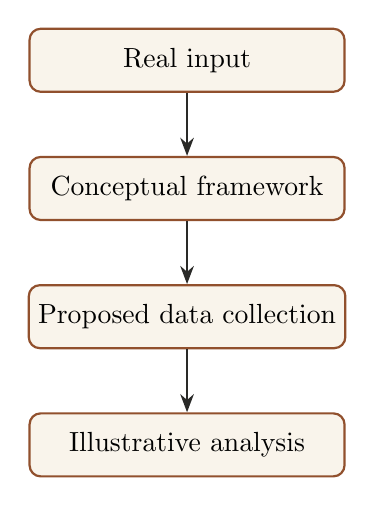
\begin{tikzpicture}[node distance=8mm,box/.style={rectangle,rounded corners,draw=clay,fill=sand,thick,align=center,minimum width=4.0cm,minimum height=8mm},arrow/.style={-{Stealth[length=2.3mm]},thick,draw=ink}]
\node[box] (a) {Real input};
\node[box,below=of a] (b) {Conceptual framework};
\node[box,below=of b] (c) {Proposed data collection};
\node[box,below=of c] (d) {Illustrative analysis};
\draw[arrow] (a) -- (b);
\draw[arrow] (b) -- (c);
\draw[arrow] (c) -- (d);
\end{tikzpicture}
\caption{Premium Draft Demo workflow}
\end{figure}

\section{Illustrative Findings}

\begin{tcolorbox}[noticebox,title={Simulated Findings Warning}]
\simulated{} The findings in this section are illustrative. They demonstrate writing structure and must be replaced by real anonymized evidence before any real submission.
\end{tcolorbox}

\subsection{Theme 1: [theme]}

\begin{tcolorbox}[quotebox,title={Simulated excerpt, P01-demo}]
[simulated quote]
\end{tcolorbox}

[Claim-first interpretation with boundary.]

\section{Discussion}

\subsection{Theoretical Implications}

[Explain what the illustrative analysis would mean for the paper's core concepts if supported by real data. Keep the verbs calibrated: simulated material can illustrate a possible mechanism, but only real evidence can show a finding.]

\subsection{Methodological Implications}

[Explain why the chosen route fits the claim type. For qualitative-led work, clarify why interviews, cases, artifacts, or archives are needed before any questionnaire can be treated as more than an auxiliary tool.]

\subsection{Practice Or Education Implications}

[Explain how the proposed study could inform teaching, design practice, policy, management, communication, heritage work, or another practical setting. Keep recommendations conditional until real evidence exists.]

\subsection{Boundary Conditions}

[State where the argument may fail: limited cases, narrow target journals, unverified literature, simulated quotes, convenience sampling, missing ethics approval, or absent longitudinal evidence.]

\subsection{From Demo To Real Study}

[Summarize the minimum viable real-study plan: verify 8-12 core papers, select 2-3 cases, confirm ethics route, run 2 pilot interviews, collect 6-8 initial formal interviews, revise the codebook once, and replace every DRAFT-SIM marker.]

\section{Conclusion}

[Restate the central contribution, the demo boundary, and the real-data steps needed next.]

\appendix
\section{Demo Interview Protocol}

\proposed{} [Add study purpose, inclusion/exclusion criteria, consent, recording, withdrawal, anonymization, RQ mapping, questions, and probes.]

\section{Demo Questionnaire Module}

\begin{table}[htbp]
\centering
\caption{Demo construct-item table}
\begin{tabularx}{\textwidth}{P{3cm}Y Y}
\toprule
\textbf{Construct} & \textbf{Demo item} & \textbf{Boundary} \\
\midrule
[construct] & [item] & [source and pilot needed] \\
\bottomrule
\end{tabularx}
\end{table}

\section{Demo Codebook}

\begin{table}[htbp]
\centering
\caption{Demo codebook}
\begin{tabularx}{\textwidth}{P{3cm}P{2.4cm}Y}
\toprule
\textbf{Code} & \textbf{Type} & \textbf{Definition} \\
\midrule
[code] & preset/open/negative & [definition] \\
\bottomrule
\end{tabularx}
\end{table}


\section*{Reference Boundary}

\begin{tcolorbox}[greenbox,title=Verified references used for claims]
[List only sources that have been read or provided in enough detail to support a specific sentence. If none are verified, write: No verified reference list is generated in this demo.]
\end{tcolorbox}

\begin{tcolorbox}[mainbox,title=Candidate references to verify]
[List metadata-only or candidate sources here. These may guide the next reading step but must not be treated as evidence for manuscript claims.]
\end{tcolorbox}

\begin{tcolorbox}[noticebox,title=Citation TODOs]
[List conceptual claims, method claims, and empirical gap claims that still need verified sources before submission.]
\end{tcolorbox}
\end{document}
